\documentclass[12pt,a4paper]{article}

% Essential packages
\usepackage[margin=1in]{geometry}
\usepackage{graphicx}
\usepackage{amsmath}
\usepackage{amssymb}
\usepackage{listings}
\usepackage[table]{xcolor}
\usepackage{hyperref}
\usepackage{titling}
\usepackage{float}
\usepackage{enumitem}
\usepackage{fancyhdr}
\usepackage{placeins}

% Additional packages for beautification
\usepackage[skins,breakable]{tcolorbox}
\usepackage{fontspec}
\usepackage{booktabs}
\usepackage{mdframed}
\usepackage{caption}
\usepackage{soul}
\usepackage{verbatim}
\usepackage{tikz}
\usetikzlibrary{positioning, arrows.meta, shapes.geometric}

\usepackage{array}
\setlength{\tabcolsep}{6pt}

% Color definitions
\definecolor{titleblue}{RGB}{0,76,151}
\definecolor{myblue}{RGB}{25,25,112}
\definecolor{lightbluegray}{RGB}{220,230,245}  
\definecolor{mygreen}{RGB}{0,128,0}
\definecolor{mygray}{RGB}{245,245,245}

% Custom tcolorbox styles
\tcbset{
    mybox/.style={
        enhanced,
        colback=myblue!3,
        colframe=myblue,
        arc=2mm,
        boxrule=0.8pt
    }
}

\newtcolorbox{mytitledbox}[1]{
    enhanced,
    colback=myblue!3,
    colframe=titleblue!50,
    arc=2mm,
    boxrule=1.1pt,
    title={\textcolor{white}{\textbf{#1}}},
    coltitle=white,
    fonttitle=\bfseries,
    colbacktitle=titleblue!50
}

\newtcolorbox{solutionbox}{
    enhanced,
    colback=lightbluegray!80,  
    colframe=titleblue!50,     
    arc=1.5mm,                
    boxrule=0.15pt,            
    top=2mm,                 
    bottom=2mm,
    before=\vspace{2mm},       % Space before box
    after=\vspace{2mm},        % Space after box
    breakable                  % For long solutions
}

% Header and footer setup
\pagestyle{fancy}
\fancyhf{}
\renewcommand{\headrulewidth}{0.8pt}
\renewcommand{\footrulewidth}{0.4pt}
\fancyhead[L]{\textsf{\textcolor{myblue}{Microprocessors Laboratory}}}
\fancyhead[R]{\textsf{\textcolor{myblue}{Lab 3 Report}}}
\fancyfoot[C]{\thepage}
\setlength{\headheight}{14.5pt}
\addtolength{\topmargin}{-2.5pt}

% Custom section styling
\usepackage{titlesec}
\titleformat{\section}
  {\normalfont\Large\bfseries\color{myblue}}
  {\thesection}{1em}{}[\titlerule]
\titleformat{\subsection}
  {\normalfont\large\bfseries\color{myblue}}
  {\thesubsection}{1em}{}
\titleformat{\subsubsection}
  {\normalfont\normalsize\bfseries\color{myblue}}
  {\thesubsubsection}{1em}{}

\title{
    \vspace*{2cm}
    \Huge\textbf{\textsf{Microprocessors Laboratory Report}}\\
    \vspace{0.4cm}
    \Large\textsf{Lab 3: Autonomous Environmental Control System with DHT11 Sensor}
    \vspace{1cm}
    \rule{\textwidth}{1pt}
}

\author{
    \Large\begin{tabular}{rl}
        \textbf{Fraidakis Ioannis}\\
    \end{tabular}
}

\date{\Large\textsf{June 2025}}

% Listing style for code
\lstdefinestyle{mystyle}{
    backgroundcolor=\color{mygray},
    commentstyle=\color{mygreen},
    keywordstyle=\color{blue},
    numberstyle=\tiny\color{gray},
    stringstyle=\color{purple},
    basicstyle=\ttfamily\small,
    breakatwhitespace=false,
    breaklines=true,
    captionpos=b,
    keepspaces=true,
    numbers=left,
    numbersep=5pt,
    showspaces=false,
    showstringspaces=false,
    showtabs=false,
    tabsize=2,
    frame=single,
    framesep=5pt,
    framerule=0.5pt,
    framexleftmargin=6pt,
    framexrightmargin=6pt,
    framextopmargin=4pt,
    framexbottommargin=4pt,
}
\lstset{style=mystyle}

\begin{document}
\maketitle

\section{Introduction}

\begin{tcolorbox}[mybox]
This laboratory exercise implements an autonomous environmental control system using the ARM NUCLEO M4 microcontroller (STM32F411RE). The system demonstrates advanced microcontroller programming concepts including sensor interfacing, dual-mode operation and multi-level alert management.

The system features a DHT11 temperature-humidity sensor interface, touch sensor-driven mode switching, comprehensive UART command interface, and sophisticated alert management with panic reset functionality. The implementation showcases interrupt-driven architecture, real-time environmental monitoring, and user-interactive control systems.

The following sections detail the system architecture, implementation methodology, testing procedures, and insights gained from developing this comprehensive embedded environmental control solution.
\end{tcolorbox}

\newpage

\section{System Overview}

\subsection{Hardware Components}
The system integrates the following hardware components:

\begin{tcolorbox}[mybox]
\begin{itemize}[label=\textcolor{myblue}{$\bullet$}, itemsep=1.5mm]
    \item \textbf{DHT11 Sensor:} Connected to GPIO pin \texttt{PC\_0}, providing digital temperature and humidity measurements using 1-wire communication protocol.
    \item \textbf{Status LED:} Connected to GPIO pin \texttt{PB\_0}, used for visual alert indication with programmable blinking patterns.
    \item \textbf{Touch Sensor:} Connected to GPIO pin \texttt{PC\_1}, configured with rising trigger interrupt for mode switching.
    \item \textbf{UART Interface:} Provides bidirectional communication for user authentication, command processing, and data output at 115200 baud rate.
\end{itemize}
\end{tcolorbox}

\subsection{Software Architecture}

\subsubsection{Key Data Structures}

\begin{mytitledbox}{Data Structures}
\begin{itemize}[label=\textcolor{myblue}{$\circ$}, itemsep=1.5mm]
    \item \textbf{System State Management:} Global \texttt{volatile} variables manage operational modes, authentication states, and configuration parameters. The \texttt{volatile} keyword ensures correct ISR-main loop data sharing.

    \item \textbf{UART Receive Queue:} A \texttt{Queue} structure buffers incoming UART characters, decoupling interrupt reception from main loop processing.

    \item \textbf{Sensor Data Storage:} Floating-point variables store the most recent temperature and humidity readings.

    \item \textbf{Authentication Context:} Secure storage for user credentials and AEM (student ID) with proper buffer management and security considerations.
\end{itemize}
\end{mytitledbox}

\subsubsection{Operational Modes}
The system operates using a dual-mode architecture with authentication gate:

\begin{tcolorbox}[mybox]
\begin{itemize}[label=\textcolor{myblue}{$\blacktriangleright$}, itemsep=1.5mm]
    \item \textbf{Authentication Phase}: Password verification followed by AEM capture with secure input handling and visual feedback.
    \item \textbf{Mode A (Normal)}: Standard environmental monitoring with configurable frequency and display options.
    \item \textbf{Mode B (Alert)}: Enhanced monitoring with LED alerts, threshold detection, and automatic recovery mechanisms.
\end{itemize}
\end{tcolorbox}

\begin{center}
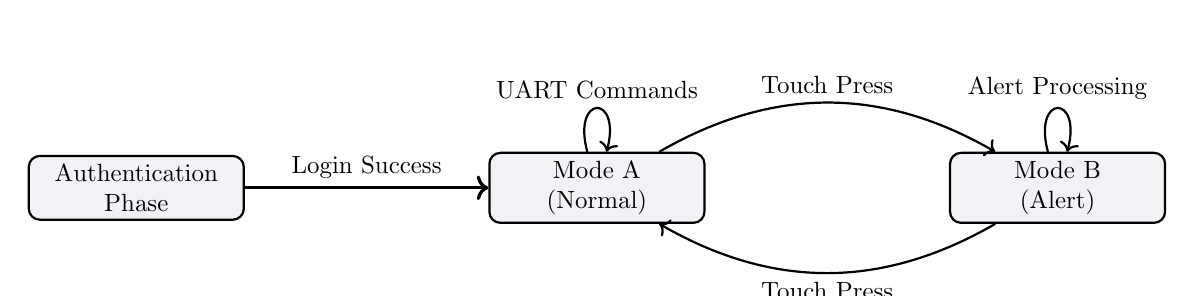
\begin{tikzpicture}[node distance=6.5cm, auto, thick, scale=0.9, transform shape]
    % Nodes
    \node[draw, rounded corners, fill=myblue!6, text width=2.8cm, align=center] (auth) {Authentication\\Phase};
    \node[draw, rounded corners, fill=myblue!6, text width=2.8cm, align=center, right of=auth] (normal) {Mode A\\(Normal)};
    \node[draw, rounded corners, fill=myblue!6, text width=2.8cm, align=center, right of=normal] (alert) {Mode B\\(Alert)};
    
    % Edges
    \draw[->, very thick] (auth) to node[above] {Login Success} (normal);
    \draw[->, thick] (normal) to[bend left] node[above] {Touch Press} (alert);
    \draw[->, thick] (alert) to[bend left] node[below] {Touch Press} (normal);
    \draw[->, thick] (normal) to[loop above] node[above] {UART Commands} ();
    \draw[->, thick] (alert) to[loop above] node[above] {Alert Processing} ();
\end{tikzpicture}
\end{center}

\subsubsection{Interrupt Service Routines}
Four main interrupt handlers orchestrate system operations:

\begin{tcolorbox}[mybox]
\begin{itemize}[label=\textcolor{myblue}{$\blacktriangleright$}, itemsep=1.5mm]
    \item \textbf{timer\_callback()}: Manages periodic sensor readings, LED blinking timing, and system timing base with 1-second resolution.
    \item \textbf{button\_press\_callback()}: Handles touch sensor events with debouncing, mode switching logic, and frequency update calculations.
    \item \textbf{uart\_receive\_callback()}: Processes incoming UART characters with queue buffering and ASCII validation.
\end{itemize}
\end{tcolorbox}

\section{Implementation Details}

\subsection{UART Command Interface}
The system provides comprehensive command processing:

\begin{tcolorbox}[mybox]
\begin{center}
\begin{tabular}{|l|l|l|}
\hline
\textbf{Command} & \textbf{Function} & \textbf{Range/Constraints} \\
\hline
'a' & Increase frequency (decrease period) & Minimum: 2 seconds \\
\rowcolor{lightbluegray!55}
'b' & Decrease frequency (increase period) & Maximum: 10 seconds \\
'c' & Toggle display mode & Temperature/Humidity/Both \\
\rowcolor{lightbluegray!55}
'd' & Show detailed system status & All parameters \\
'status' & Compact system information & Quick overview \\
\rowcolor{lightbluegray!55}
Ctrl+C & Clear screen and refresh & Terminal reset \\
Ctrl+X & Safe system termination & Graceful shutdown \\
\hline
\end{tabular}
\end{center}
\end{tcolorbox}

\subsection{Enhanced Console Interface}
The system features a sophisticated UART interface with:

\begin{tcolorbox}[mybox]
\begin{itemize}[label=\textcolor{myblue}{$\star$}, itemsep=1.5mm]
    \item \textbf{ANSI Color Coding:} Different colors for various message types
    \item \textbf{Animated Headers:} Professional-looking bordered headers for messages
    \item \textbf{Progress Indicators:} Visual feedback during authentication and processing
    \item \textbf{Input Restoration:} Smart terminal handling that preserves user input during system messages
\end{itemize}
\end{tcolorbox}


\section{Testing}

\begin{mytitledbox}{Test Scenarios}
\begin{tabular}{@{}p{0.25\textwidth}p{0.3\textwidth}p{0.4\textwidth}@{}}
\toprule[1.5pt]
\textbf{\textcolor{myblue}{Test Category}} & \textbf{\textcolor{myblue}{Test Case}} & \textbf{\textcolor{myblue}{Expected Outcome}} \\
\midrule[0.8pt]
Authentication & Correct password "2025" & Proceed to AEM input stage \\
\rowcolor{lightbluegray!55} 
Authentication & Incorrect password & Error message, re-prompt \\
Authentication & AEM input "10736" & Successful login, menu display \\
\rowcolor{lightbluegray!55}
Sensor Reading & Normal conditions & Temperature/humidity display \\
Mode Switching & Touch sensor press & Toggle between Mode A/B \\
\rowcolor{lightbluegray!55}
Frequency Control & Command 'a' & Increase frequency (min 2s) \\
Frequency Control & Command 'b' & Decrease frequency (max 10s) \\
\rowcolor{lightbluegray!55}
AEM Frequency & 3rd touch press & Update from AEM last 2 digits \\
Display Toggle & Command 'c' & Cycle through T/H/Both modes \\
\rowcolor{lightbluegray!55}
Alert System & Temp > 25°C in Mode B & LED blinking activation \\
Alert Recovery & 5 normal readings & LED stops, alert cleared \\
\rowcolor{lightbluegray!55}
Panic Reset & Temp > 35°C (3 times) & System reset triggered \\
Status Display & Command 'd' or 'status' & Detailed system information \\
\rowcolor{lightbluegray!55}
Terminal Control & Ctrl+C & Screen clear, menu refresh \\
Safe Shutdown & Ctrl+X & Graceful program termination \\
\bottomrule[1.5pt]
\end{tabular}
\end{mytitledbox}

\subsection{Validation Methodology}

\begin{mytitledbox}{Validation Steps}
\begin{itemize}[label=\textcolor{myblue}{$\checkmark$}, itemsep=1.5mm]
    \item \textbf{Sensor Accuracy:} Verify DHT11 readings against reference measurements and validate checksum integrity.
    \item \textbf{Mode Transitions:} Test touch sensor responsiveness and proper state transitions between modes.
    \item \textbf{Alert Thresholds:} Validate alert activation/deactivation with controlled environmental conditions.
    \item \textbf{Command Processing:} Verify all UART commands function correctly with proper error handling.
\end{itemize}
\end{mytitledbox}

\subsection{Challenges and Solutions}

\begin{mytitledbox}{Implementation Challenges}
\begin{enumerate}[label=\textcolor{myblue}{\textbf{\arabic*.}}, itemsep=1.5mm]    

    \item \textbf{DHT11 Timing Critical Sections:} 
    The DHT11 sensor requires microsecond-precise timing for proper communication. Any interrupt during the critical reading phase could disrupt the timing and cause data corruption or communication failure.
    
    \begin{solutionbox}
    \textit{Solution:} Implemented critical sections during DHT11 communication by temporarily disabling interrupts using \texttt{\_\_disable\_irq()} and \texttt{\_\_enable\_irq()} around timing-sensitive operations. Additionally, used dedicated timing functions with precise delay mechanisms to ensure protocol compliance. The sensor reading is scheduled during low-activity periods to minimize interrupt conflicts.
    \end{solutionbox}
    
\end{enumerate}
\end{mytitledbox}

\section{Conclusion}

\begin{tcolorbox}[mybox]
This laboratory project successfully demonstrates the implementation of a sophisticated autonomous environmental control system. The solution integrates multiple advanced concepts including sensor interfacing, dual-mode operation, secure authentication, and intelligent alert management.

Key achievements include robust DHT11 sensor communication with precise timing control, comprehensive user authentication with security considerations, flexible operational modes with touch sensor control, and a multi-level alert system with automatic recovery capabilities.

The implementation showcases professional embedded software development practices including modular architecture, interrupt-driven design, proper error handling, and user-friendly interface design. The system provides a solid foundation for real-world environmental monitoring applications with potential extensions for IoT connectivity and advanced analytics.

\end{tcolorbox}

\section*{References}
\begin{itemize}[label=\textcolor{myblue}{$\triangleright$}]
    \item STM32F411RE Microcontroller Reference Manual
    \item DHT11 Temperature-Humidity Sensor Datasheet
    \item Touch Sensor Datasheet

\end{itemize}

\end{document}